\documentclass{beamer}
\usepackage[utf8]{inputenc}
\usepackage[UKenglish]{babel}
\usepackage[UKenglish]{isodate}
\usepackage{graphicx}
\usepackage{tikz}
\usepackage{phaistos}
\usepackage{wasysym}

\usetikzlibrary{shapes}
\usetheme{Boadilla}
\beamertemplatenavigationsymbolsempty
\author{Paulius Dilkas}
\title{Modelling Movement with Bigraphs}
%s\subtitle{}
\institute[]{School of Computing Science}
\date{12th September 2018}

\newcommand\pro{\item[\textcolor{green}{$+$}]}
\newcommand\con{\item[\textcolor{red}{$-$}]}
\providecommand\longdoublearrowRHD{\mathrel\LHD\joinrel\relbar\joinrel\relbar\joinrel\mathrel\RHD}

\begin{document}
\maketitle
\tikzstyle{every picture}+=[remember picture]

\begin{frame}{Motivation}
  \begin{columns}[t]
    \column{0.5\textwidth}
    \centering
    \begin{overlayarea}{\textwidth}{0.5\textheight}
      \includegraphics<-2>[width=\textwidth]{uav.jpg}
      \includegraphics<3->[width=\textwidth]{drone.jpg}
    \end{overlayarea}
    \begin{overlayarea}{\textwidth}{0.5\textheight}
      \includegraphics<-3>[width=\textwidth]{underwater.jpg}
      \includegraphics<4->[width=\textwidth]{boat.png}
    \end{overlayarea}
    \column{0.5\textwidth}
    \centering
    \begin{overlayarea}{\textwidth}{0.5\textheight}
      \includegraphics<1>[width=\textwidth]{ground.jpg}
      \includegraphics<2->[width=\textwidth]{car.jpg}
    \end{overlayarea}
    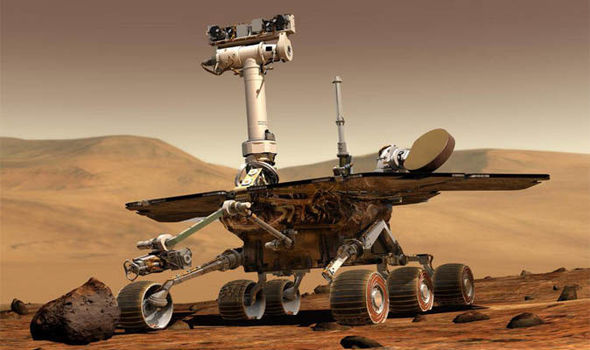
\includegraphics[width=\textwidth]{rover.jpg}
  \end{columns}
\end{frame}

\begin{frame}{Markov Decision Process}
  \begin{figure}
    \centering
    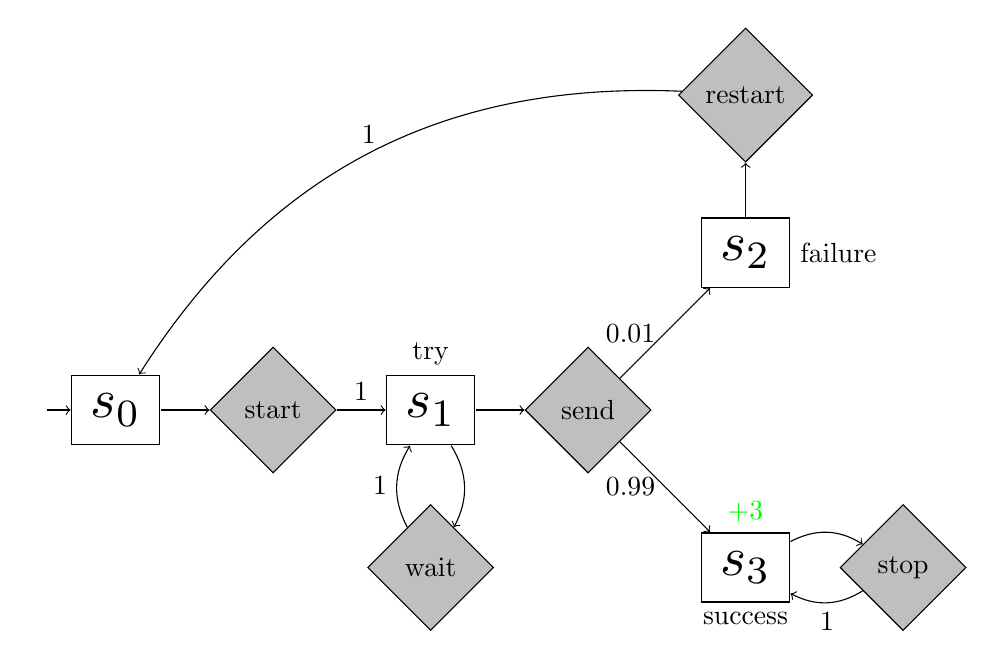
\begin{tikzpicture}[state/.style={rectangle, draw, scale=2},
      action/.style={diamond, draw, fill=lightgray, minimum size=1.6cm}]
      \node(origin) at (-1, 0){};
      \node[state](s0) at (0, 0){$s_0$};
      \node[action](start) at (2, 0){start};
      \node[state,label=try](s1) at (4, 0){$s_1$};
      \node[action](wait) at (4, -2){wait};
      \node[action](send) at (6, 0){send};
      \node[state,label={right:failure}](s2) at (8, 2){$s_2$};
      \node[action](restart) at (8, 4){restart};
      \node[state,label={below:success},label={above:\textcolor{green}{+3}}](s3) at (8, -2){$s_3$};
      \node[action](stop) at (10, -2){stop};
      \draw[-{>[scale=2]}] (s0) edge (start);
      \draw[-{>[scale=2]}] (start) edge node[above] {$1$} (s1);
      \draw[-{>[scale=2]},bend left] (s1) edge (wait);
      \draw[-{>[scale=2]},bend left] (wait) edge node[left] {$1$} (s1);
      \draw[-{>[scale=2]}] (s1) edge (send);
      \draw[-{>[scale=2]}] (send) edge node[left] {$0.01$} (s2);
      \draw[-{>[scale=2]}] (send) edge node[left] {$0.99$} (s3);
      \draw[-{>[scale=2]}] (s2) edge (restart);
      \draw[-{>[scale=2]},bend right] (restart) edge node[above] {$1$} (s0);
      \draw[-{>[scale=2]},bend left] (s3) edge (stop);
      \draw[-{>[scale=2]},bend left] (stop) edge node[below] {$1$} (s3);
      \draw[-{>[scale=2]}] (origin) edge (s0);
    \end{tikzpicture}
  \end{figure}
\end{frame}

\begin{frame}{Collecting Objects in a Grid}
  \begin{itemize}
  \item Each cell is either visited or unvisited.
  \item When entering an unvisited cell, with probability $p$ the agent may
    receive an object.
  \item Once a set number of objects is collected, the agent heads home.
  \end{itemize}
\end{frame}

\begin{frame}{Collecting Objects in a Grid}
  \begin{figure}
    \centering
    
\begin{tikzpicture}[overlay]
      \only<1>{
        \fill[fill=black!20!white] (-1, -2) rectangle (2, 2);
        \fill[fill=black!20!white] (-2, -1) rectangle (-1, 2);
        \draw[step=1cm,very thin] (-2, -2) grid (2, 2);
        \node at (-1.5, -1.6) {\PHchild};
      }
      \only<2>{
        \fill[fill=black!20!white] (-1, -2) rectangle (2, 2);
        \fill[fill=black!20!white] (-2, 0) rectangle (-1, 2);
        \draw[step=1cm,very thin] (-2, -2) grid (2, 2);
        \node at (-1.5, -0.6) {\PHchild};
      }
      \only<3>{
        \fill[fill=black!20!white] (-1, -2) rectangle (2, 2);
        \fill[fill=black!20!white] (-2, 1) rectangle (-1, 2);
        \draw[step=1cm,very thin] (-2, -2) grid (2, 2);
        \node at (-1.4, 0.4) {\PHchild};
        \node at (-1.8, 0.4) {$\bigstar$};
      }
      \only<4>{
        \fill[fill=black!20!white] (-1, -2) rectangle (2, 2);
        \fill[fill=black!20!white] (-2, 1) rectangle (-1, 2);
        \draw[step=1cm,very thin] (-2, -2) grid (2, 2);
        \node at (-1.4, -0.6) {\PHchild};
        \node at (-1.8, -0.6) {$\bigstar$};
      }
      \only<5>{
        \fill[fill=black!20!white] (0, -2) rectangle (2, 2);
        \fill[fill=black!20!white] (-2, 1) rectangle (-1, 2);
        \fill[fill=black!20!white] (-1, 0) rectangle (0, 2);
        \fill[fill=black!20!white] (-1, -2) rectangle (0, -1);
        \draw[step=1cm,very thin] (-2, -2) grid (2, 2);
        \node at (-0.4, -0.6) {\PHchild};
        \node at (-0.8, -0.8) {$\bigstar$};
        \node at (-0.8, -0.5) {$\bigstar$};
      }
      \only<6>{
        \fill[fill=black!20!white] (0, -2) rectangle (2, 2);
        \fill[fill=black!20!white] (-2, 1) rectangle (-1, 2);
        \fill[fill=black!20!white] (-1, 0) rectangle (0, 2);
        \fill[fill=black!20!white] (-1, -2) rectangle (0, -1);
        \draw[step=1cm,very thin] (-2, -2) grid (2, 2);
        \node at (-1.4, -0.6) {\PHchild};
        \node at (-1.8, -0.8) {$\bigstar$};
        \node at (-1.8, -0.5) {$\bigstar$};
      }
      \only<7>{
        \fill[fill=black!20!white] (0, -2) rectangle (2, 2);
        \fill[fill=black!20!white] (-2, 1) rectangle (-1, 2);
        \fill[fill=black!20!white] (-1, 0) rectangle (0, 2);
        \fill[fill=black!20!white] (-1, -2) rectangle (0, -1);
        \draw[step=1cm,very thin] (-2, -2) grid (2, 2);
        \node at (-1.4, -1.6) {\PHchild};
        \node at (-1.8, -1.8) {$\bigstar$};
        \node at (-1.8, -1.5) {$\bigstar$};
      }
    \end{tikzpicture}
  \end{figure}
\end{frame}

\begin{frame}{Bigraphs}
  \tikzstyle{na} = [baseline=-0.5ex]
  \begin{columns}
    \begin{column}{0.5\textwidth}
      \begin{itemize}
      \item<2-> Region \tikz[na] \coordinate (t-region);
      \item<3-> Nodes \tikz[na] \coordinate (t-node);
      \item<4-> Site \tikz[na] \coordinate (t-site);
      \item<5-> Links \tikz[na] \coordinate (t-link);
      \end{itemize}
    \end{column}
    \begin{column}{0.5\textwidth}
      \begin{figure}
        \centering
        \begin{tikzpicture}
          \node {\includegraphics[width=\textwidth]{../models/agent1/home.pdf}};
          \path (-3, 2) coordinate (region);
          \path (-2.4, 0.6) coordinate (node1);
          \path (-2.4, -0.5) coordinate (node2);
          \path (-2.2, -2) coordinate (site);
          \path (-1.9, 2) coordinate (link1);
          \path (-0.8, 2.1) coordinate (link2);
          \path (2.5, 2.1) coordinate (link3);
        \end{tikzpicture}
      \end{figure}
    \end{column}
  \end{columns}
  \begin{tikzpicture}[overlay]
    \path[->]<2-> (t-region) edge[blue] (region);
    \path[->]<3-> (t-node) edge[blue] (node1);
    \path[->]<3-> (t-node) edge[blue] (node2);
    \path[->]<4-> (t-site) edge[blue] (site);
    \path[->,bend left=60]<5-> (t-link) edge[blue] (link1);
    \path[->,bend left=70]<5-> (t-link) edge[blue] (link2);
    \path[->,bend left=80]<5-> (t-link) edge[blue] (link3);
  \end{tikzpicture}
\end{frame}

\begin{frame}{Transition System}
  \begin{figure}
    \centering
    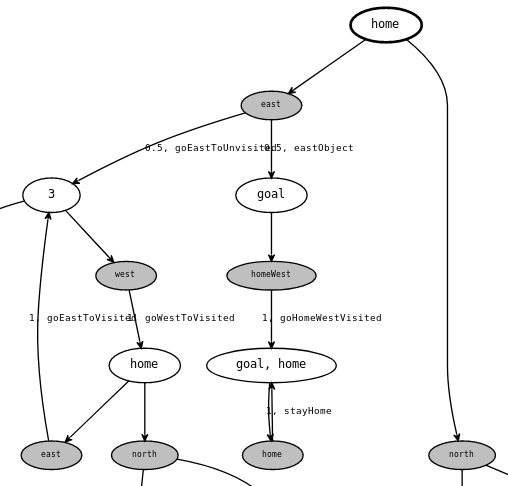
\includegraphics[scale=0.17]{../models/agent1/ts.pdf}
  \end{figure}
\end{frame}

\begin{frame}{Transition System}
  \begin{figure}
    \centering
    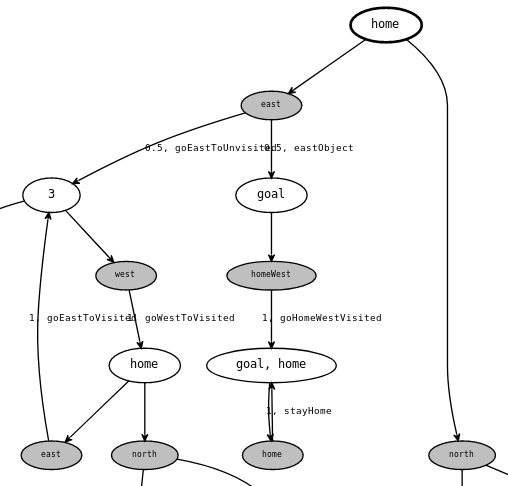
\includegraphics[clip, trim=15cm 35cm 20cm 0cm, width=\textwidth]{../models/agent1/ts.pdf}
  \end{figure}
\end{frame}

\begin{frame}{A Tale of Schr\"{o}dinger's Wall...}
  \begin{figure}
    \centering
    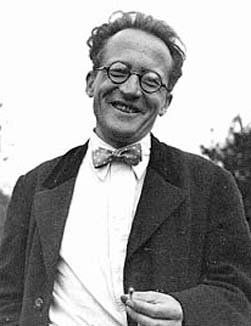
\includegraphics[height=\textheight]{schrodinger.jpg}
  \end{figure}
\end{frame}

\begin{frame}{A Tale of Schr\"{o}dinger's Wall...}
  \begin{figure}
    \centering
    
\begin{tikzpicture}[overlay]
      \only<1>{
        % outside walls
        \draw (-0.25, 0.5) -- (-1.5, 0.5) -- (-1.5, 1.5) -- (1.5, 1.5) -- (1.5, 0.5) -- (0.25, 0.5);
        % background grid
        \draw[gray,very thin] (-0.5, 1.5) -- (-0.5, 0.5);
        \draw[gray,very thin] (0.5, 1.5) -- (0.5, 0.5);
        % agent
        \node at (-1, 0.9) {\PHchild};
        % door
        \draw[brown,ultra thick] (-0.25, 0.5) -- (0.25, 0.5);
      }
      \only<2>{
        % outside walls
        \draw (-0.25, 0.5) -- (-1.5, 0.5) -- (-1.5, 1.5) -- (1.5, 1.5) -- (1.5, 0.5) -- (0.25, 0.5);
        % background grid
        \draw[gray,very thin] (-0.5, 1.5) -- (-0.5, 0.5);
        \draw[gray,very thin] (0.5, 1.5) -- (0.5, 0.5);
        % agent
        \node at (0, 0.9) {\PHchild};
        % door
        \draw[brown,ultra thick] (-0.25, 0.5) -- (0.25, 0.5);
      }
      \only<3-4>{
        % outside walls
        \draw (1.5, 0.5) -- (1.5, -1.5) -- (-0.5, -1.5) -- (-0.5, 0.5) -- (-1.5, 0.5) -- (-1.5, 1.5) -- (1.5, 1.5) -- (1.5, 0.5) -- (0.5, 0.5);
        % probabilistic wall
        \draw[red,ultra thick,dashed] (0.5, 0.5) -- (0.5, -0.5);
        % background grid
        \draw[gray,very thin] (-0.5, 1.5) -- (-0.5, 0.5);
        \draw[gray,very thin] (0.5, 1.5) -- (0.5, 0.5);
        \draw[gray,very thin] (-0.5, -0.5) -- (1.5, -0.5);
        \draw[gray,very thin] (0.5, -0.5) -- (0.5, -1.5);
        % agent
        \node at (0, 0.9) {\PHchild};
        % door
        \draw[dotted] (-0.25, 0.5) arc (180:270:0.5cm);
        \draw[brown,ultra thick] (0.25, 0) -- (0.25, 0.5) node[right,  near start]{};
        \draw (-0.5, 0.5) -- (-0.25, 0.5);
        \draw (0.25, 0.5) -- (0.5, 0.5);
        % target
        \node at (1, 0) {$\bigstar$};
      }
      \only<4>{
        \draw[->, ultra thick, green] (0, 0.5) -- (0, 0) -- (0.8, 0);
        \draw[->, ultra thick, green] (0, 0.5) -- (0, -1) -- (1, -1) -- (1, -0.2);
      }
    \end{tikzpicture}
  \end{figure}
\end{frame}

\begin{frame}{Reaction Rules}
  \begin{columns}
    \begin{column}{0.45\textwidth}
      \begin{figure}
        \centering
        \includegraphics[width=\textwidth]{../models/agent2/goIn_lhs.pdf}
      \end{figure}
    \end{column}
    \begin{column}{0.1\textwidth}
      $\longdoublearrowRHD$
    \end{column}
    \begin{column}{0.45\textwidth}
      \begin{figure}
        \centering
        \includegraphics[width=\textwidth]{../models/agent2/goIn_rhs.pdf}
      \end{figure}
    \end{column}
  \end{columns}
\end{frame}

\begin{frame}{Conclusions}
  \begin{itemize}
    \pro A direct visual representation of the modelled situation
    \pro Easy to represent complicated spatial structures and uncertainty about
    them
    \pro Succinct and easy to modify
    \con Some simple ideas are impossible or hard to implement
    \con Not every aspect of a model can be exported for quantitative analysis
    \item More work to be done on probabilistic space
  \end{itemize}
\end{frame}

\end{document}